\documentclass[headings=standardclasses,headings=big,oneside,a4paper,openany,12pt]{scrbook}

\newcommand {\e}[1]{\mathrm{~#1}}
\newcommand {\E}[1]{\times 10^{#1}}
\newcommand {\vars}{$\Delta E$ and $M_{BC}$}
\newcommand {\btbii}{\texttt{B2BII}}
\newcommand {\decaya}{$B \to K K \ell \nu$}
\newcommand {\decayb}{$B^+ \to K^+ K^- \ell^+ \nu$}

%\usepackage{biblatex}
%\bibliography{mybib.bib} 
\usepackage[slovene,english]{babel}% Recommended
\usepackage{csquotes}% Recommended
\usepackage[sorting=none,firstinits=true,backend=bibtex]{biblatex}
\addbibresource{mybib.bib}% Syntax for version >= 1.2

\usepackage{paralist}
\usepackage{caption}
\usepackage{cancel}

\usepackage{longtable}

\setlength{\parskip}{1em}%
\setlength{\parindent}{0cm}

\usepackage{titling}
\usepackage{amsmath,amssymb,amsfonts,nicefrac}
\usepackage{graphicx}
\usepackage{color}
\usepackage{float}
\usepackage{mathtools}
\allowdisplaybreaks
\usepackage[pdftex,colorlinks=true,citecolor=blue,linkcolor=black,urlcolor=blue,bookmarks=true]{hyperref}
\usepackage{dictsym}
\usepackage{braket}
\usepackage{slashed}
\DeclareMathOperator{\arcsinh}{arcsinh}
\usepackage{enumerate}
\usepackage{array}
\setlength{\extrarowheight}{.5ex}

\usepackage{lineno}
\linenumbers

\usepackage{subfigure}


\begin{document}
\begin{otherlanguage}{slovene}
\chapter{Povzetek doktorskega dela}

\section{Uvod}
Fizika delcev je eden od stebrov fizike, z mo"cnimi koreninami, ki segajo vse do za"cetka 20. stoletja. Natan"cni eksperimenti in preverljiva teorija so pokazali, da vesolje sestoji iz osnovnih delcev in nosilcev interakcij. Osnovne delce delimo na kvarke ($u$, $d$, $s$, $c$, $b$, $t$) in leptone, ki so nadaljnje razdeljeni na nabite leptone ($e$, $\mu$, $\tau$) in pa nevtrine ($\nu_e$, $\nu_\mu$, $\nu_\tau$). Nosilci treh (od "stirih) osnovnih interakcij, s katerimi se ukvarjamo na tem podro"cju, so fotoni ($\gamma$) za elektromagnetno, gluoni ($g$) za mo"cno in nabiti- ($W^\pm$) ter nevtralni ($Z^0$) bozoni za "sibko interakcijo. Vsi delci in njihovi zrcalni partnerji, antidelci (ozna"ceni z $~\bar {}~$), imajo maso, ki jim jo dolo"ca Higgsov bozon ($H$). Vse delce ter interakcije med njimi opisuje Standardni model, ki je osrednja teorije fizike visokih energij. Kvarke lahko zdru"zujemo v kombinacije oblike $q_1 q_2 q_3$ (hadroni) ali pa $q_1 \bar{q}_2$ (mezoni), med katere sodijo tudi protoni in nevtroni, ki jih opazimo v naravi. Poleg omenjenih dolgo-"zive"cih delcev pa obstajajo tudi te"zji, manj stabilni delci, ki preko zgoraj na"stetih interakcij razpadejo v la"zje, stabilnej"se. Raziskovanje tak"snih procesov s pomo"cjo pospe"sevalnikov in trkalnikov nam omogo"ca spoznavanje zakonov vesolja danes pa vse do njegovega za"cetka.

Osrednji del doktorske disertacije predstavljajo meritve razpadov mezonov $B$, delcev, ki so sestavljeni iz te"zkega kvarka $b$ in enega od lahkih kvarkov $u$ ali $d$. Ena bolj presenetljivih lastnosti vesolja je kr"sitev simetrije $CP$, t.j. kombinacije simetrij konjugacije naboja ($C$) in prostorske inverzije ($P$). Simetrija $CP$ nakazuje, da so fizikalni procesi delcev in zrcalni procesi antidelcev enaki, kar pa danes vemo, da ne dr"zi v celoti in poznamo procese, ki to simetrijo kr"sijo. Kr"sitev simetrije $CP$ je tesno povezana s "sibko interakcijo, to pa predstavlja na"so motivacijo za "studijo mezonov $B$, saj "sibki razpadi predstavljajo ve"cji del vseh razpadov mezonov $B$.

Edinstvena lastnost "sibke interakcije je, da lahko spreminja tip oziroma t.i. okus kvarkov, medtem ko ga ostale interakcije ohranjajo. Tak"sni procesi so opisani s prehodno matriko CKM (Cabibbo-Kobayashi-Maskawa) \cite{cabibbo1963unitary,kobayashi1973cp}
\begin{equation}
V_{CKM} = \begin{bmatrix}
    V_{ud} & V_{us} & V_{ub}\\
	V_{cd} & V_{cs} & V_{cb}\\
	V_{td} & V_{ts} & V_{tb}
\end{bmatrix}.
\end{equation}
Unitarnost matrike CKM nam omogo"ca, da iz nje izlu"s"cimo matemati"cne identitete, od katerih je ena pomembnej"sih
\begin{equation}
V_{ud}V_{ub}^* + V_{cd}V_{cb}^* + V_{td}V_{tb}^* = 0,
\end{equation}
poznana pod imenom unitarni trikotnik, saj predstavlja zaklju"cen vektor treh to"ck v kompleksni ravnini, kot prikazuje Slika \ref{fig:ut_si}. Parametri matrike CKM niso dolo"cljivi s strani teorije, temve"c jih moramo dolo"citi z eksperimentalnimi meritvami tako, da najdemo procese, ki so tesno povezani s stranicami in koti unitarnega trikotnika. Na tak na"cin lahko preverimo, "ce je oblika trikotnika konsistentna, kar predstavlja dober test Standardnega modela, oziroma "ce so potencialno prisotni kak"sni novi procesi, ki jih "se ne poznamo, in jih kolektivno imenujemo "nova fizika". Dodatna motivacija za "studijo mezonov $B$ je ta, da velik dele"z njihovih razpadov predstavlja koristne procese za meritev unitarnega trikotnika.
\begin{figure}[H]
\centering
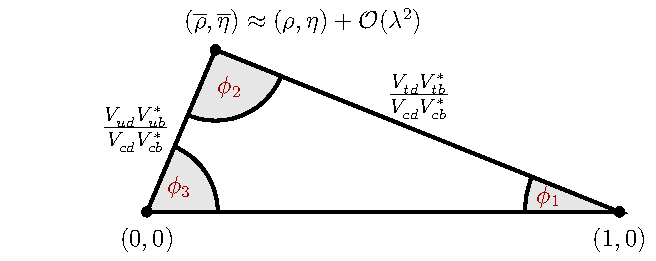
\includegraphics[scale=1]{texfig/UT_Triangle}
\caption{Unitarni trikotnik s parametri $\lambda,~\eta,~\rho$ and $A$ (slednji ni prikazan), ki predstavljajo proste parametre matrike CKM.} %TODO: Wolf. param. 
\label{fig:ut_si}
\end{figure}

Procesi, ki jih "studiramo v tej analizi, so tesno povezani z elementom $V_{ub}$ matrike CKM, saj le-ta opisuje prehode kvarkov $b \to c$. Od vseh elementov, je absolutna vrednost tega elementa najmanj"sa, relativna napaka pa najve"cja, zato meritve iz tega podro"cja potencialno omogo"cajo najve"c izbolj"save. Tak"sni prehodi kvarkov so prisotni v nečarobnih (t.j. brez kvarkov $c$) semi-leptonskih razpadih mezonov $B$ oblike 
\begin{equation}
B^+ \to X_u^0 \ell^+ \nu_\ell,
\end{equation}
kjer $X_u^0$ predstavlja ne"carnobne mezone, $\ell$ pa je eden od nabitih leptonov. Frekvenco razpadov, ki je tesno povezana z elementom $V_{ub}$, opi"semo z ena"cbo
\begin{equation}
\mathrm{d} \Gamma \propto G_F^2 \vert V_{ub} \vert ^2 \vert L^\mu \langle X_u \vert \bar u \gamma_u \frac{1}{2} (1-\gamma_5) b \vert B \rangle \vert ^2,
\end{equation}
kjer $G_F$ predstavlja Fermijevo konstanto, $L^\mu$ leptonski tok, izraz v Diracovih oklepajih pa hadronski tok. V tak"snih prehodih $\vert V_{ub} \vert ^2$ predstavlja verjetnost za prehod $b \to u$.

Meritev elementa $V_{ub}$ je mo"zna na ekskluziven in inkluziven na"cin, kjer pri prvi metodi opravljamo meritve v specifi"cno definirana kon"cna stanja, kot na primer $B \to \pi \ell \nu$, pri drugi metodi pa opravljamo meritev s kupno kon"cno stanje oblike $B \to X_u \ell \nu$. Obe metodi potekata preko razli"cnih pristopov in se soo"cata z razli"cnimi tezavami, kar pomeni, da sta oba kon"cna rezultata nekorelirana. Rezultata obeh meritev imata tudi zelo podobno natan"cnost, medtem ko se srednja vrednost le deloma ujema. Rezultata se razlikujeta s signifikanco $3\sigma$, kar predstavlja ve"cjo te"zavo znotraj podro"cja. Trenutni svetovni povpre"cji \cite{Amhis:2016xyh} ekskluzivne (iz razpadov $B^0 \to \pi^- \ell^+ \nu$) in inkluzivne meritve (GGOU kolaboracija \cite{Gambino:2007rp}) sta
\begin{align}
&\vert V_{ub} \vert_{\mathrm{e.}} = \left(3.65 \pm 0.09 \pm 0.11\right)\E{-3},\\
&\vert V_{ub} \vert_{\mathrm{i.}}^{\mathrm{GGOU}} = \left(4.52 \pm 0.15~{}^{+0.11}_{-0.14}\right)\E{-3},
\end{align}
kjer prva in druga napaka predstavljata eksperimentalno in teoretsko napako. Rezultati inkluzivnih meritev so praviloma ve"cji kot rezultati ekskluzivnih. Razlogov za neujemanje je lahko ve"c, od nepoznanih napak pri eksperimentu ali teoriji, do prispevkov nove fizike.

V tej analizi se osredoto"camo na enega od mo"znih razlogov za zgoraj omenjeno neujemanje, konkretneje za razpad \decayb, ki je strukturno precej podoben razpadu $B \to \pi \ell \nu$ za razliko produkcije para kvarkov $s \bar s$ ki se potem hadronizira v nove delce, kot prikazuje Slika \ref{feynman}. V inkluzivnih meritvah ne"carobnih semi-leptonskih razpadov mezonov $B$ se standardno uporablja $K$-veto, t.j. selekcija, kjer zahtevamo, da v kon"cnem stanju nimamo mezonov $K$ (sestava $q \bar s,~q \in [u,d]$), poznanih tudi pod imenom kaoni. Kaoni v kon"cnem stanju nakazujejo na pogost prehod kvarkov $b \to c \to s$, ki pa jih ho"cemo v analizah prehodov $b \to u$ zatreti. V primeru na"se analize imamo v kon"cnem stanju 2 kaona s prehodom $b \to u$, kar pomeni, da tak"sni razpadi niso upo"stevani v inkluzivnih meritvah, "ceprav bi morali biti. Cilj "studije je dolo"citi pogostost razpadov \decayb~s prehodom $b\to u$ in s tem oceniti, kak"sen potencialen efekt ima lahko neupo"stevanje teh razpadov na inkluzivno meritev elementa $V_{ub}$. V nadaljevanju bo razpad \decayb~zaradi enostavnosti zapisan kot \decaya.
\begin{figure}[H]
\centering
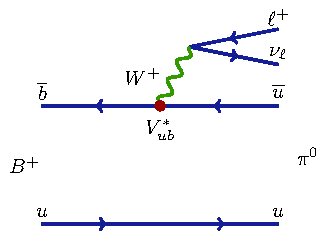
\includegraphics{texfig/B2pilnu}
\hspace{1cm}
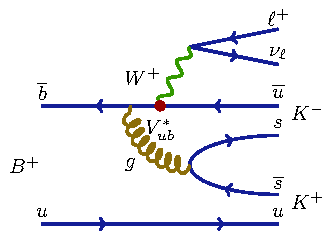
\includegraphics{texfig/B2KKlnu}
\caption{Feynmanovi diagrami za razpada $B^+ \to \pi^0 \ell^+ \nu_\ell$ (levo) in $B^+ \to K^- K^+ \ell^+ \nu_\ell$ (desno).}
\label{feynman}
\end{figure}

\section{Experimentalna postavitev}
\subsection{Trkalnik KEKB}
\subsection{Detektor Belle}
\section{Postopek analize}
\section{Sistematske negotovosti}
\section{Kon\v cni rezultat}
\end{otherlanguage}
\end{document}


